\documentclass[11pt,letterpaper]{article}

% include figures
\usepackage{graphicx}
\usepackage{caption,subcaption}
% get nice colors
\usepackage{xcolor}

% change default font to Palatino (looks nicer!)
\usepackage[latin1]{inputenc}
\usepackage{mathpazo}
\usepackage[T1]{fontenc}
% load some useful math symbols/fonts
\usepackage{latexsym,amsfonts,amsmath,amssymb,wasysym}
% be able to insert code
\usepackage{listings}

% comfort package to easily set margins
\usepackage[top=1in, bottom=1in, left=1in, right=1in]{geometry}

% spacing after a paragraph
\setlength{\parskip}{.15cm}
% indentation at the top of a new paragraph
\setlength{\parindent}{0.0cm}
% make units not slanted in math mode
\newcommand{\unit}[1]{\ensuremath{\, \mathrm{#1}}}

\begin{document}

\begin{center}
\Large
Ay190 -- Worksheet 16\\
Daniel DeFelippis\\
Date: \today
\end{center}

%%
%%
%% I worked with Scott Barenfeld
%%
%% All python code can be found in the ws16 directory in my repository
%%
%%

\section*{1D Finite Volume Hydro Code}

\section{}

This code solves a bunch of local Riemann problems by interpolating the midpoint of
a pair of gridpoints using some kind of "reconstruction" and then calculating flux 
differences and integrating forwards in time.

For convenience in keeping track of all of the variables, the program defines
a class called "mydata". In it, it distinguishes between primitive variables (density 
$\rho$, velocity $v$, internal energy per mass $\epsilon$, and pressure $P$) and 
conserved variables $\rho$, $\rho v$, and $\rho\epsilon + \frac{1}{2}\rho v^2$. The
equation of state used is $P = (\gamma - 1)\rho\epsilon$. 

First, the program sets up the grid with three ghost points on either side to 
let it calculate local Riemann problems on the edges. It then sets the initial conditions.
The function "apply\_bcs" applies boundary values to the ghost points by 
simply setting them equal to the last interior point. 

It then calculates the smallest possible time step by taking the distance between two
gridpoints, dividing it by the maximum of the sum and difference of that grid point's 
velocity and speed of sound, and choosing the minimum of the resulting $\Delta t_i$'s.

There are three different types of reconstruction the program defines to interpolate
the values of the variables at the interface. Piecewise constant, the simplest, sets the
left and right values of the variables at the interface to be their values at the grid
points. Total Variational Diminishing minmod reconstruction uses an estimate of the slope
at the interface to calculate what the values there should be. If the slope at the 
two grid points around it are different signs, it sets the slope to 0 and this method
reduces to the piecewise constant method at that point. The monotonized central method 
is a higher order method and uses a more accurate estimate of the slope. It should 
theoretically give the most accurate result.

Finally, at each iteration, the program calculates the flux at each interface by first
finding the min and max characteristic speeds ($s_{min}$ and $s_{max}$ respectively) 
there (from the left and right grid points). The characteristic speeds are eigenvalues 
of the euler equations given by 
\begin{align*}
\lambda_1 &= v - c_s \\
\lambda_2 &= v \\
\lambda_3 &= v + c_s
\end{align*}
It then needs to calculate the numerical fluxes $F^L_j$ and $F^R_j$ (from the left 
and right) with the code
\lstinputlisting[language=Python, firstline=272, lastline=279]{ws16.py}
which are equations taken from IV.5.40 in the notes. With the numerical fluxes and
characteristic speeds, the flux at each interface $x_{i+1/2}$ is given by 
$$ f_j(x_{i+1/2}) =  \frac{s_{max}F^L_j - s_{min}F^R_j + s_{min}s_{max}(q^R_j - q^L_j)}{s_{max} - s_{min}} $$
where $j$ goes from 1 to 3 and represents that number Euler equation, and $q_j$ is the conserved quantity corresponding to the $j^{th}$ Euler equation. Finally, it calculates
the flux difference (FD) at each grid point using the values at the interfaces:
$$ FD_i = \frac{1}{\Delta x_i} [f(x_{i+1/2}) - f(x_{i-1/2})]. $$

Every 10 iterations, the program plots the density profile of the solution. Some 
of these plots are shown below in figures~\ref{fig:it0and80} to \ref{fig:it640and720} which
use piecewise constant reconstruction. 

Just like ws15, we see the expected zones: the first and fifth are constant with the initial
densities as the value, and there is a rarefaction zone as well as clear contact and shock 
close-to-vertical lines.

\begin{figure}[bth]
\centering
\begin{subfigure}{.5\textwidth}
  \centering
  \includegraphics[width=.95\linewidth]{out_0.pdf}
  \caption*{Piecewise Constant (PC) Density profile: Iteration 0}
  \label{fig:sub1}
\end{subfigure}%
\begin{subfigure}{.5\textwidth}
  \centering
  \includegraphics[width=.95\linewidth]{out_80.pdf}
  \caption*{Iteration 80}
  \label{fig:sub2}
\end{subfigure}
\caption{}
\label{fig:it0and80}
\end{figure}

\begin{figure}[bth]
\centering
\begin{subfigure}{.5\textwidth}
  \centering
  \includegraphics[width=.95\linewidth]{out_160.pdf}
  \caption*{Iteration 160}
  \label{fig:sub3}
\end{subfigure}%
\begin{subfigure}{.5\textwidth}
  \centering
  \includegraphics[width=.95\linewidth]{out_240.pdf}
  \caption*{Iteration 240}
  \label{fig:sub4}
\end{subfigure}
\caption{}
\label{fig:it160and240}
\end{figure}

\begin{figure}[bth]
\centering
\begin{subfigure}{.5\textwidth}
  \centering
  \includegraphics[width=.95\linewidth]{out_320.pdf}
  \caption*{Iteration 320}
  \label{fig:sub5}
\end{subfigure}%
\begin{subfigure}{.5\textwidth}
  \centering
  \includegraphics[width=.95\linewidth]{out_400.pdf}
  \caption*{Iteration 400}
  \label{fig:sub6}
\end{subfigure}
\caption{}
\label{fig:it320and400}
\end{figure}

\begin{figure}[bth]
\centering
\begin{subfigure}{.5\textwidth}
  \centering
  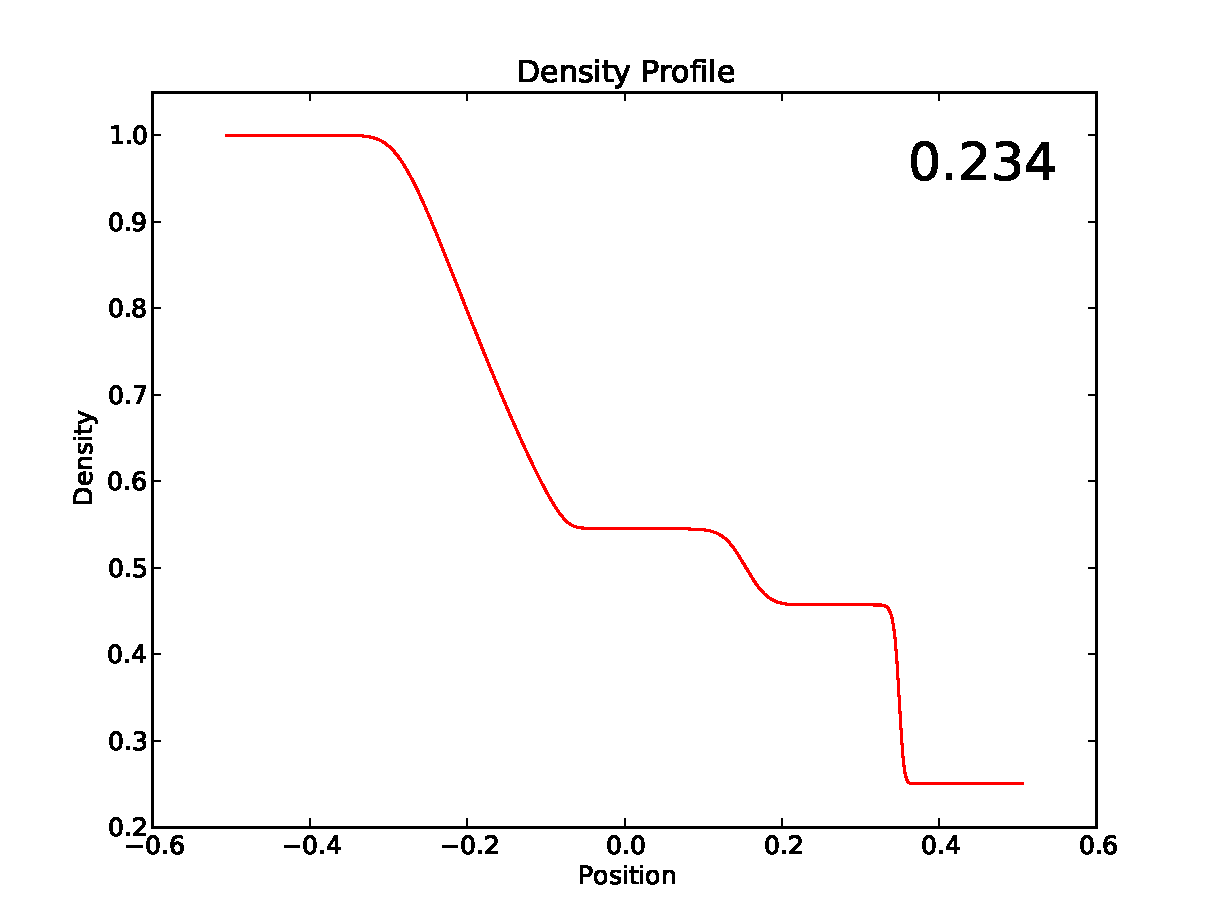
\includegraphics[width=.95\linewidth]{out_480.pdf}
  \caption*{Iteration 480}
  \label{fig:sub5}
\end{subfigure}%
\begin{subfigure}{.5\textwidth}
  \centering
  \includegraphics[width=.95\linewidth]{out_560.pdf}
  \caption*{Iteration 560}
  \label{fig:sub6}
\end{subfigure}
\caption{}
\label{fig:it480and560}
\end{figure}

\begin{figure}[bth]
\centering
\begin{subfigure}{.5\textwidth}
  \centering
  \includegraphics[width=.95\linewidth]{out_640.pdf}
  \caption*{Iteration 640}
  \label{fig:sub5}
\end{subfigure}%
\begin{subfigure}{.5\textwidth}
  \centering
  \includegraphics[width=.95\linewidth]{out_720.pdf}
  \caption*{Iteration 720}
  \label{fig:sub6}
\end{subfigure}
\caption{}
\label{fig:it640and720}
\end{figure}


\section{}

Plotting the density at $t=0.2$ in figure~\ref{fig:recon_density} for the three 
different reconstruction methods, we
see that as expected, the monotonized centered reconstruction produces the best result. 
The lines at about $x=0.15$ and $x=0.3$, which are supposed to be vertical, are most 
vertical using that reconstruction method.

\begin{figure}[bth]
\centering
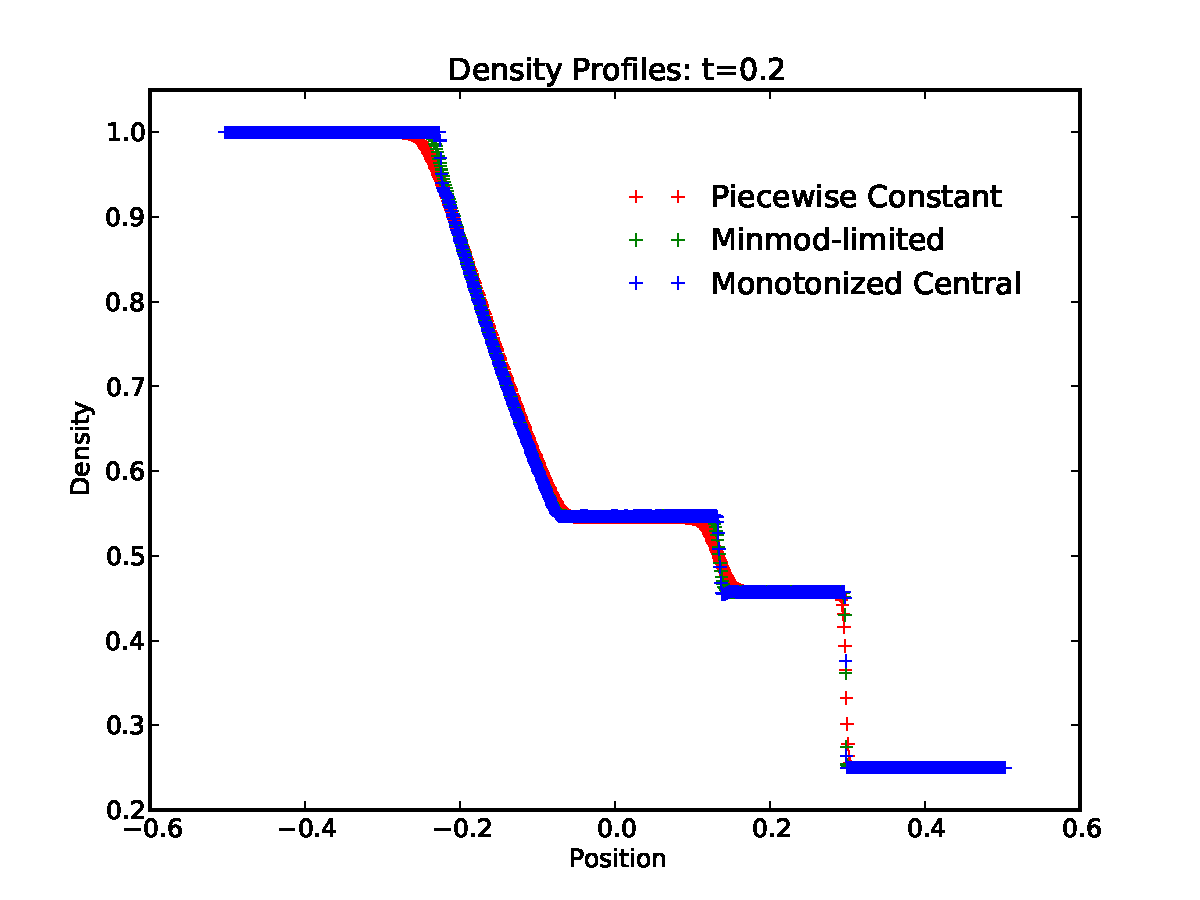
\includegraphics[width=0.75\textwidth]{reconstruction_densities.pdf}
\caption{Density profiles of Piecewise Linear, TVD-minmod,
         and TVD-MC2 reconstruction methods at $t=0.2$.}
\label{fig:recon_density}
\end{figure}



\section{}

We now compare the best reconstruction method (MC) to the results from the previous
worksheet (the SPH solver and the exact solver). We plot the density, velocity, and 
pressure profiles in figures~\ref{fig:density}, \ref{fig:velocity}, and~\ref{fig:pressure}
respectively. The MC reconstruction method is indeed very good, as it almost completely 
covers up the exact solution at $t=0.2$. The only location that seems to be innacurate
is the beginning of the rarefaction zone around $x=-0.2$. Notably, there are no
curved edges like in the SPH solution, and there's no pressure instability spike at
$x=0.15$.  

\begin{figure}[bth]
\centering
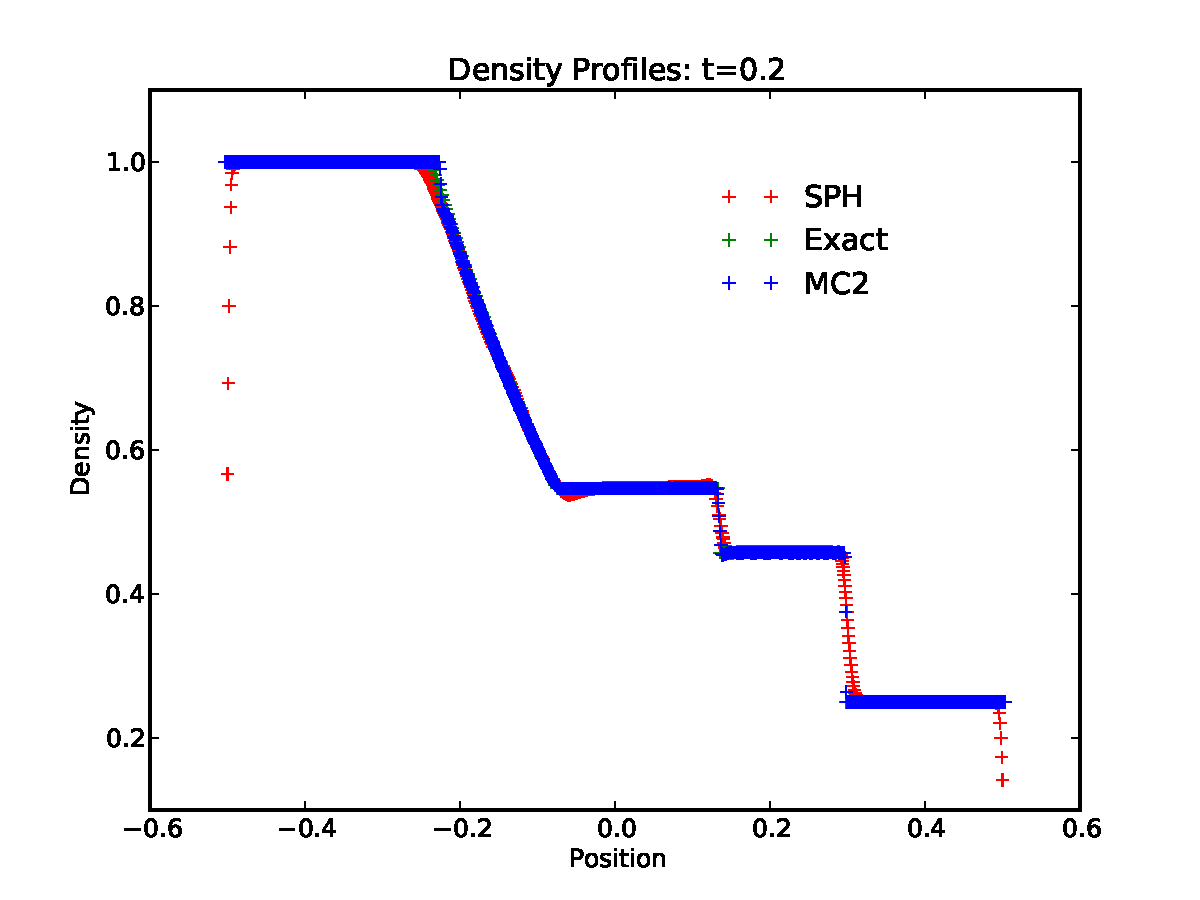
\includegraphics[width=0.75\textwidth]{density_with_ws15.pdf}
\caption{Density profiles of SPH, exact Riemann solver,
         and TVD-MC2 reconstruction at $t=0.2$.}
\label{fig:density}
\end{figure}

\begin{figure}[bth]
\centering
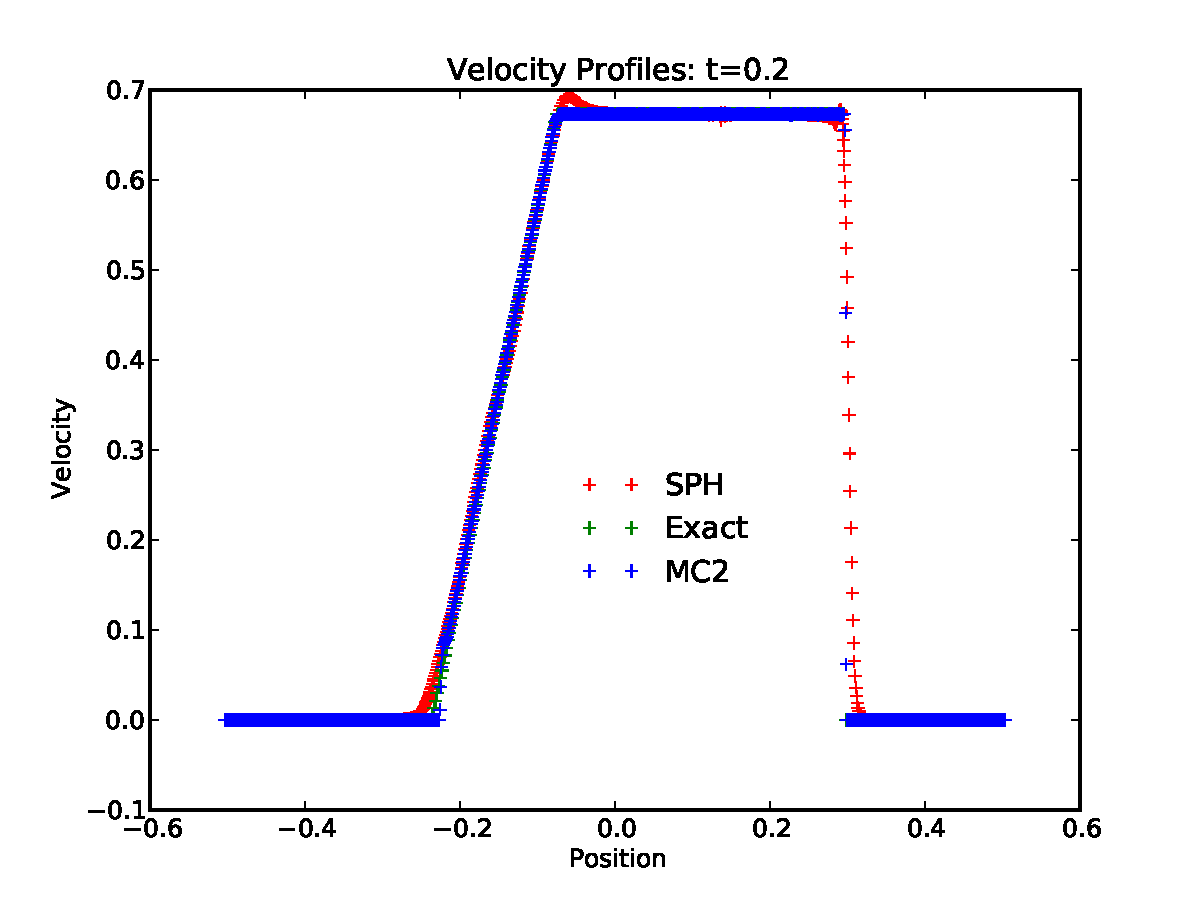
\includegraphics[width=0.75\textwidth]{velocity_with_ws15.pdf}
\caption{Velocity profiles of SPH, exact Riemann solver,
         and TVD-MC2 reconstruction at $t=0.2$.}
\label{fig:velocity}
\end{figure}

\begin{figure}[bth]
\centering
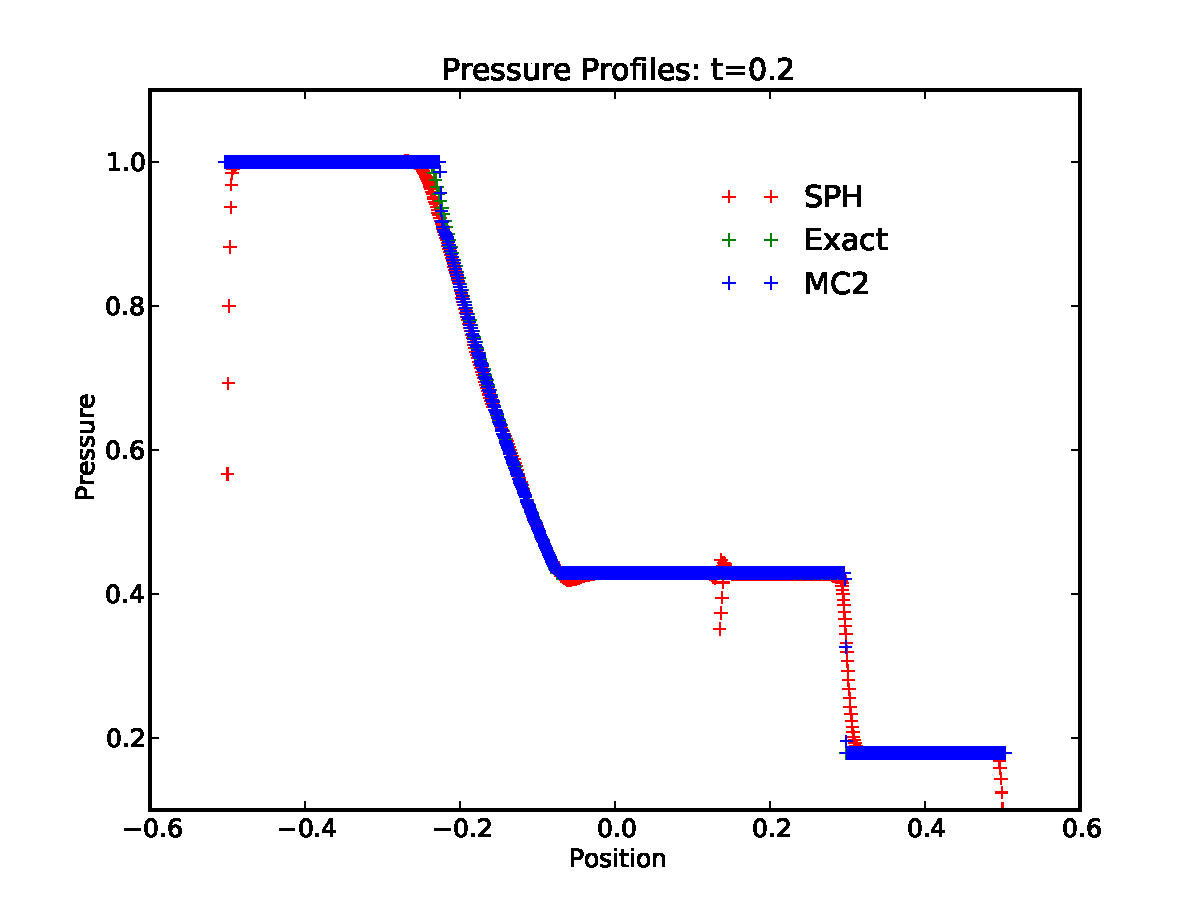
\includegraphics[width=0.75\textwidth]{pressure_with_ws15.pdf}
\caption{Pressure profiles of SPH, exact Riemann solver,
         and TVD-MC2 reconstruction at $t=0.2$.}
\label{fig:pressure}
\end{figure}


\end{document}
